\begin{frame}{Normalizing flows}
    Normalizing flows represent an approach for defining invertible and differentiable transformations of probability distributions.
    They are widely used for:
    \begin{itemize}
        \item generative modeling \citep[\textbf{GLOW}, \textbf{Real NVP}]{kingma_glow_2018, dinh_density_2017}
        \item variational inference (\cite{rezende_variational_2016, berg_sylvester_2019})
    \end{itemize}
\end{frame}

\begin{frame}{Implementation of the Normalizing Flows}
    As implementation of the normalizing flows, I use the coupling block \citep[Real NVP]{dinh_density_2017} from the Framework for Easily Invertible Architectures (FrEIA) \footnote{https://github.com/VLL-HD/FrEIA}.
    \begin{figure}
        \centering
        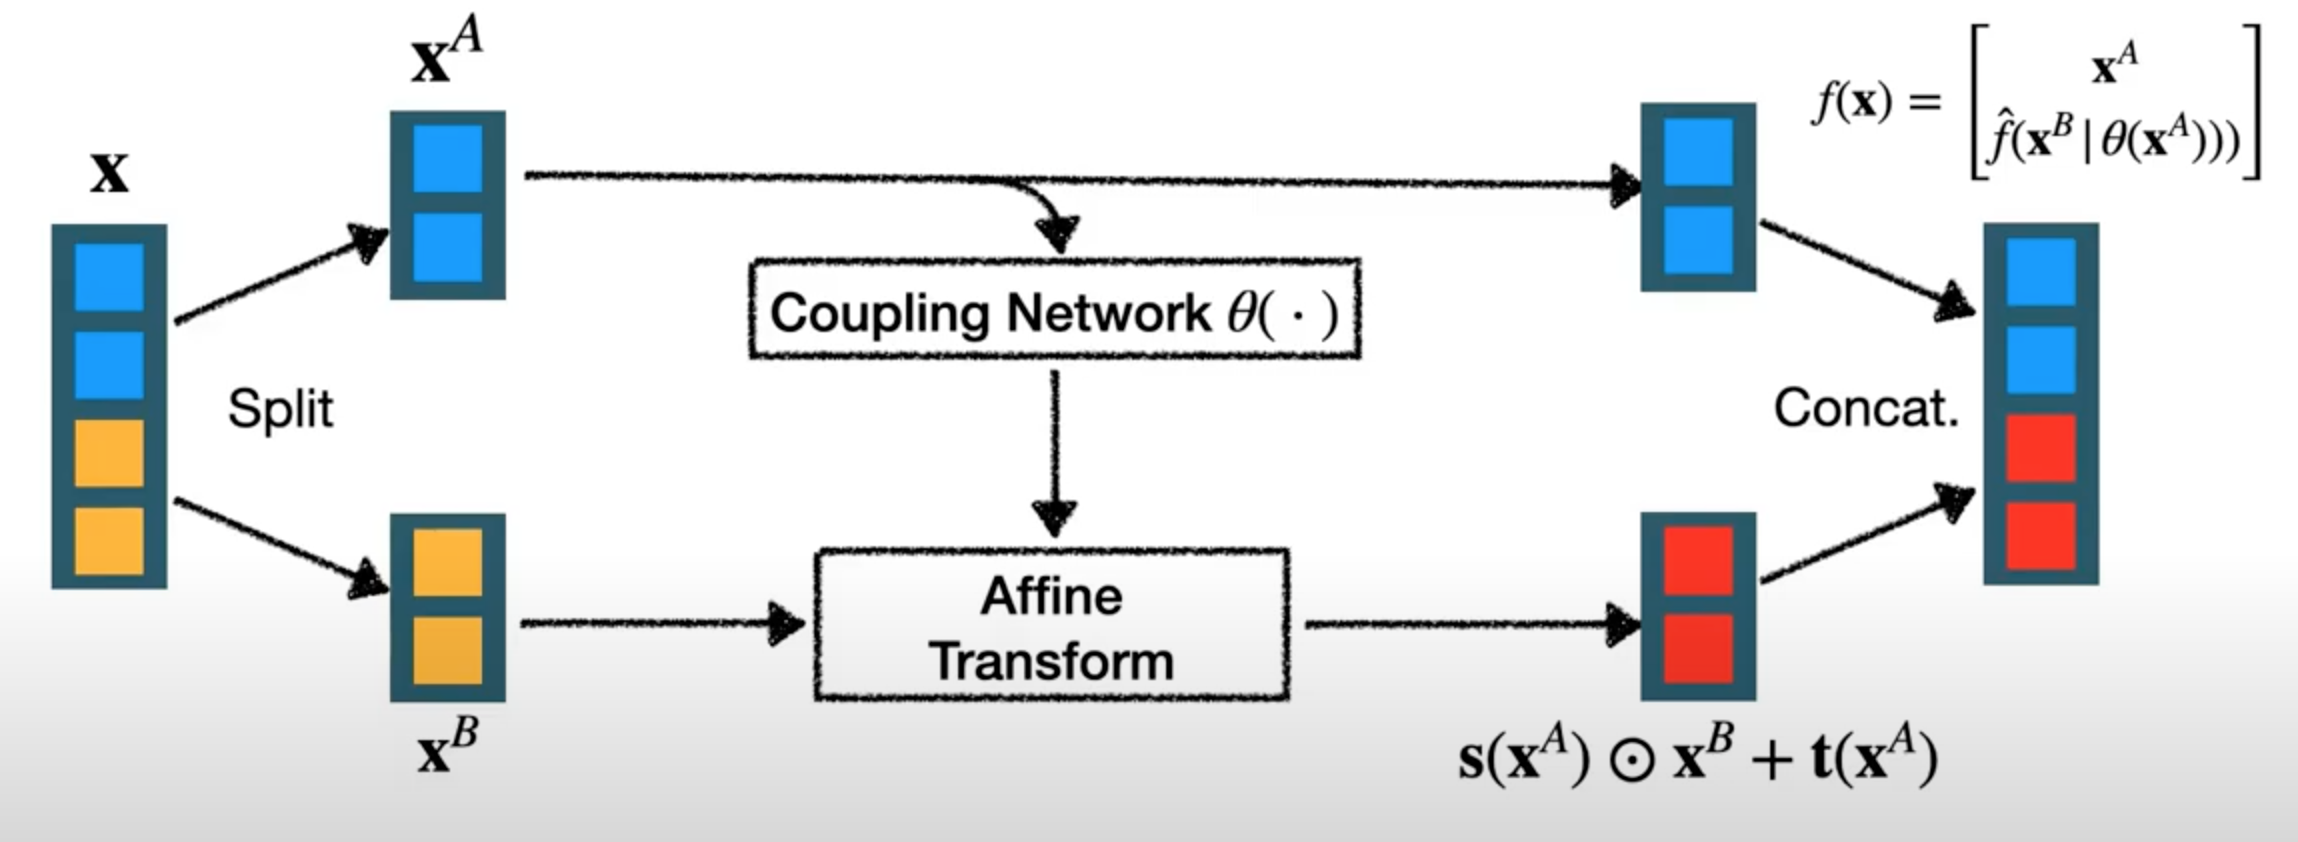
\includegraphics[width = 0.8\textwidth]{midterm_presentation/coupling_flow}
        \caption{\tiny{Taken from https://youtu.be/u3vVyFVU\_lI}}
    \end{figure}
\end{frame}

\begin{frame}{The polymnist dataset}
    \begin{figure}
        \centering
        \includegraphics[width=0.8\textwidth]{data/polymnist_example}
    \end{figure}
    Properties:
    \begin{itemize}
        \item Very simple class representation (almost the same across all modalities and very simple)
        \item More difficult modality specific representation (background of \textit{Mod 0} and \textit{Mod 2} is more complex)
    \end{itemize}
\end{frame}

\begin{frame}{Difficulties}
    The main difficulty comes from the fact that the $f$-mean of Normal distributions is not a Normal distribution.\\
    $\rightarrow$ The KL-divergence is hard to compute.\\
    \begin{equation*}
        \log p_{\theta}(\mathbb{X}) \geq \mathcal{L}(\theta, \phi; \xset):= \mathbb{E}_{q_{\phi}(\textbf{z}|\mathbb{X})}[\log (p_{\theta}(\mathbb{X}|\textbf{z}))] - D_{KL}\biggl(  q_{\phi}(\textbf{z}|\mathbb{X})\ ||\ p_{\theta}(\textbf{z})\biggr)
    \end{equation*}
\end{frame}

\begin{frame}{KL-divergence of $f$-mean}
    \textbf{3 options}:

    \begin{enumerate}[<+->]
        \item Instead of mixing distributions $\mathcal{M}_{f_{\psi}}(\mathcal{N}(\mu _i, \sigma_i^2))$, mix the parameters:\\
        $\mu_{joint} = \mathcal{M}_{f_{\psi}}(\mu _i)$, $\sigma_{joint}^2 = \mathcal{M}_{f_{\psi}}( \sigma_i^2)$ $\rightarrow q_{\phi_{joint}} \sim \mathcal{N}\left(  f_{\mu}^{-1}(\sum ^M \frac{f_{\mu}(\mu_i)}{M}),f_{\sigma}^{-1}(\sum ^M \frac{f_{\sigma}(\sigma_i^2)}{M})\right)$
        \item Instead of computing the KL-divergence in closed form, calculate it by sampling from the posterior, i.e. compare k samples from the posterior with k samples from the prior
        \item \only<.>{Find an upper bound $ D^{\prime}_{KL} \geq D_{KL}(\mathcal{M}_{f_{\psi}}(\mathcal{N}(\mu _i, \sigma_i^2))\ ||\  p_{\theta})$}\only<+->{\sout{Find an upper bound $ D^{\prime}_{KL} \geq D_{KL}(\mathcal{M}_{f_{\psi}}(\mathcal{N}(\mu _i, \sigma_i^2))\ ||\  p_{\theta})$}}

    \end{enumerate}
\end{frame}

\begin{frame}{Parameter $f$-Mean VAE}
    \begin{figure}
        \centering
        \resizebox{0.9\textwidth}{!}{%
            \py{pytex_printonly(script='midterm_presentation/scripts/pgfm_graph.py', data = '')}
        }
    \end{figure}

    \begin{small}
        \begin{equation*}
            \log p_{\theta}(\mathbb{X}) \geq \eqlpgfm
        \end{equation*}

        \begin{equation*}
            \text{with:}\ \tilde{q}_{\phi_{12}} \sim \mathcal{N}\left(  f_{\mu}^{-1}(\frac{f_{\mu}(\mu_1) + f_{\mu}(\mu_2)}{2}),f_{\sigma}^{-1}(\frac{f_{\sigma}(\sigma_1^2) + f_{\sigma}(\sigma_2^2)}{2})\right)
        \end{equation*}

    \end{small}

\end{frame}

\begin{frame}{Parameter $f$-Mean VAE}
    \begin{figure}
        \centering
        \resizebox{0.9\textwidth}{!}{%
            \py{pytex_printonly(script='midterm_presentation/scripts/pgfm_graph_.py', data = '')}
        }
    \end{figure}
\end{frame}

\begin{frame}{Mixture of Parameter $f$-Mean VAE}
    \begin{figure}
        \centering
        \resizebox{0.9\textwidth}{!}{%
            \py{pytex_printonly(script='midterm_presentation/scripts/mopgfm_graph.py', data = '')}
        }
    \end{figure}

    \begin{small}
        \begin{equation*}
            \log p_{\theta}(\mathbb{X}) \geq \eqlmopgfm
        \end{equation*}

        \begin{equation*}
            \text{with:}\ \tilde{q}_{\phi_{i}} \sim \mathcal{N}\left(  f_{\mu}^{-1}(\sum ^S _{i = 0}\frac{f_{\mu}(\mu_i)}{S}),f_{\sigma}^{-1}(\sum ^S _{i = 0}\frac{f_{\sigma}(\sigma_i^2)}{S})\right)
        \end{equation*}
    \end{small}
\end{frame}

\begin{frame}{Importance Weighted $f$-Mean VAE}
    Instead of computing the KL-divergence in closed form, calculate it by sampling from the posterior following the procedure from the importance weighted autoencoder \citep{burda_importance_2016, shi_variational_2019}.
    \begin{equation*}
        \log p(x) \geq \mathbb{E}_{z_1,\ldots,z_K \sim q_{\phi}(z|x)}\left[ \log \frac{1}{K} \sum ^K _{i=1} \frac{p_{\theta}(x|z_i)p_{\theta}(z)}{q_{\phi}(z_i| x)} \right]\\
        := \mathcal{L}_K
    \end{equation*}
\end{frame}

\begin{frame}{Known results \citep{nowozin_debiasing_2018}}
    \begin{enumerate}
        \item ELBO recovery:
        \begin{equation*}
            ELBO = \mathcal{L}_1
        \end{equation*}
        \item Consistency: $\lim _{K \rightarrow \inf} \mathcal{L}_K = \log p(x)$
        \item Stochastic monotonicity:
        \begin{equation*}
            \mathcal{L}_E = \mathcal{L}_1 \leq \mathcal{L}_2 \leq \ldots \leq \log p(x)
        \end{equation*}
    \end{enumerate}
\end{frame}

\begin{frame}{Mixture of $f$-Mean}
    \begin{figure}
        \centering
        \resizebox{0.9\textwidth}{!}{%
            \py{pytex_printonly(script='midterm_presentation/scripts/mogfm_graph.py', data = '')}
        }
    \end{figure}

    \begin{equation*}
        \mathcal{L}_{mogfm} := \mathbb{E}_{q_{\phi}(z^{\prime}|\mathbb{X})}\left[ \log p_{\theta}(\mathbb{X}|z^{\prime}) \right] - D_{KL}(q_{\phi}(z|\mathbb{X})\ ||\ P_{\theta}(z))
    \end{equation*}

    Where the KL-divergence is calculated with $K$ samples from $q_{\phi}(z|\mathbb{X})$ and from the prior $q_{\theta}$:
    \begin{equation*}
        D_{KL} = \text{mean}(\left\{ l_1,\ldots,l_N \right\}) \text{, with } l_n=y_n\cdot(\log y_n -x_n) \text{ and } x_n \sim q_{\phi}(z|\mathbb{X}); y_n \sim q_{\theta}
    \end{equation*}
\end{frame}

